%**
%*  @file  Quick Start.tex
%*  @brief   DIET Qucik Startt main file  
%*  @author  - Olivier Mornard (Olivier.Mornard@sysfera.com)
%*  @section Licence 
%*    |LICENSE|


\documentclass[12pt,a4paper]{book}
%\makeatletter
%\makeatother
\usepackage{fancyhdr}
\usepackage[headings]{fullpage}

\usepackage[pdftex]{graphicx} % Pour l'insertion d'images
\DeclareGraphicsExtensions{.jpg,.mps,.pdf,.png} % Formats d'images

\usepackage[pdftex]{thumbpdf}      % Vignettes
\usepackage{xcolor} % required for colors by hyperef
\usepackage[pdftex,                %
    bookmarks         = true,%     % Signets
    bookmarksnumbered = true,%     % Signets numérotés
    pdfpagemode       = true,%     % Signets/vignettes fermés à l'ouverture
%   pdfpagemode       = Fullscreen,
    pdfstartview      = FitV,%     % La page prend toute la hauteur
    pdfpagelayout     = SinglePage,% Vue par page
    colorlinks        = true,%     % Liens en couleur
    linkbordercolor   = white, % Couleur de la boîte sur les liens normal 
    citebordercolor   = white, % Couleur de la boîte sur les citations 
    filebordercolor   = white, % Couleur sur la boîte sur les fichiers 
    urlbordercolor    = white, % Couleur sur la boîte sur les URL
    linkcolor         = cyan, % Liens internes
    urlcolor          = blue, %  % Couleur des liens externes
    pdfborder         = {0 0 0}%   % Style de bordure : ici, pas de bordure
    ]{hyperref}%                   % Utilisation de HyperTeX


\hypersetup{ % Modifiez la valeur des champs suivants
    pdfauthor   = {DIET Team},%
    pdftitle    = {DIET Quick Start},%
    pdfsubject  = {Quick Start},%
    pdfkeywords = {DIET, Grid-RPC},%
    pdfcreator  = {PDFLaTeX},%
    pdfproducer = {PDFLaTeX}}


%\usepackage[french]{babel}
%\usepackage[latin1]{inputenc}
%\usepackage{multicol}
\usepackage{verbatim}
\usepackage{url}
\usepackage{subfigure}
\usepackage{listings}
\usepackage{xspace}
\usepackage{calc}
\usepackage{marvosym} % More symbols
\graphicspath{{./fig}}

\usepackage{pifont} % for \ding{52} dagda

\newsavebox{\logobox}
\sbox{\logobox}{
\includegraphics[scale=0.4]{fig/logo_DIET}}
\newcommand{\logo}{\usebox{\logobox}}

%%%%

\newcounter{rmq}[section]
\setcounter{rmq}{0}
\newenvironment{remarque}{\addtocounter{rmq}{1}\textbf{N.B. \thermq:}}{}

%%%%

%%%%
\renewcommand{\title}{DIET Quick Start}
%%%%

\pagestyle{fancyplain}
\fancyhead[L]{\title}
% \lhead[\fancyplain{\title}{\title}]
%       {\fancyplain{\title}{\title}}
\chead{}
\rhead[\fancyplain{\logo}{\logo}]{\fancyplain{\logo}{\logo}}

\lfoot[\fancyplain{\scriptsize{\copyright} ~INRIA, ENS-Lyon, UCBL, CNRS, SysFera}{\scriptsize{\copyright} ~INRIA, ENS-Lyon, UCBL, CNRS, SysFera}]{\fancyplain{\scriptsize{\copyright} ~INRIA, ENS-Lyon, UCBL, CNRS, SysFera}{\scriptsize{\copyright} ~INRIA, ENS-Lyon, UCBL, CNRS, SysFera}}
\cfoot[\fancyplain{}{}]{\fancyplain{}{}}
\rfoot[\fancyplain{Page~\thepage}{Page~\thepage}]
      {\fancyplain{Page~\thepage}{Page~\thepage}}


\newcommand{\ie}{\emph{i.e.,} }
\newcommand{\eg}{\emph{e.g.,} }

\newcommand{\dietj}{{\sc Diet}$_J$\xspace}
\newcommand{\sedj}{{\textit SeD}$_J$\xspace}
\newcommand{\seddiet}{{\textit SeD}$_{\sc Diet}$\xspace}
\newcommand{\sedsdiet}{{\textit SeDs}$_{\sc Diet}$\xspace}
\newcommand{\MAj}{{\textit MA}$_J$\xspace}
\newcommand{\MAsj}{{\textit MAs}$_J$\xspace}
\newcommand{\MAdiet}{{\textit MA}$_{\sc Diet}$\xspace}
\newcommand{\MAsdiet}{{\textit MAs}$_{\sc Diet}$\xspace}
\newcommand{\LAj}{{\textit LA}$_J$\xspace}
\newcommand{\LAsj}{{\textit LAs}$_J$\xspace}
\newcommand{\LAdiet}{{\textit LA}$_{\sc Diet}$\xspace}
\newcommand{\LAsdiet}{{\textit LAs}$_{\sc Diet}$\xspace}
\newcommand{\clientj}{{\textit client}$_J$\xspace}
\newcommand{\clientsj}{{\textit clients}$_J$\xspace}
\newcommand{\clientdiet}{{\textit client}$_{\sc Diet}$\xspace}
\newcommand{\dagda}{{\sc Dagda}\xspace}
\newcommand{\diet}{{\sc Diet}\xspace}
\newcommand{\dietforwarder}{{\sc Diet}Forwarder\xspace}
\newcommand{\godiet}{{\sc GoDiet}\xspace}
\newcommand{\madag}{{\sc M$A_{DAG}$}\xspace}
\newcommand{\pse}{PSE\xspace}
\newcommand{\nes}{NES\xspace}
\newcommand{\ptop}{\textit{Peer-to-Peer}}
\newcommand{\red}{\textit{Red}}
\newcommand{\sci}{Scilab}
\newcommand{\scip}{Scilab$_{//}$}
\newcommand{\scalapack}{ScaLAPACK}
\newcommand{\sed}{\textit{SeD}\xspace}
\newcommand{\seds}{\textit{SeD}s\xspace}
\newcommand{\thread}{\textit{thread}}
\newcommand{\threads}{\textit{threads}}
\newcommand{\nsl}{NetSolve}
\newcommand{\fixme}[1]{\fbox{\textsl{{\bf #1}}}}

\newcommand{\dietversion}{2.8.1}

%%%%
% Document beginning
%%%%

\begin{document}

%%%%
% First sheet
%%%%

\thispagestyle{empty}
\vspace*{3cm}
\vspace*{3cm}

\begin{center}
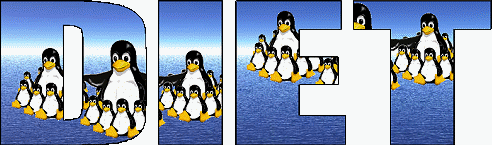
\includegraphics[scale=.5]{fig/logo_DIET_big}\\[2ex]
\textbf{\Huge Quick Start\\[2ex]}
\end{center}

\vfill

\noindent
\small{
\begin{tabular}{ll}
  \textbf{VERSION}  & \dietversion\\
  \textbf{DATE}     & Juillet 2012\\
  \textbf{PROJECT MANAGER}  & Fr\'ed\'eric \textsc{Desprez}.\\
  \textbf{EDITORIAL STAFF}  & Yves \textsc{Caniou}, Eddy
  \textsc{Caron}, Benjamin \textsc{Depardon},\\
  & Ha\"ikel \textsc{Guemar} and Ga\"el \textsc{LE-MAHEC}.\\
  \textbf{AUTHORS STAFF}    & 
\begin{minipage}[t]{12cm}
  Olivier \textsc{Mornard}.
\end{minipage} \\
  \textbf{Copyright}& INRIA, ENS-Lyon, UCBL, CNRS, SysFera
\end{tabular}\\
}

\newpage
\thispagestyle{empty}
\ 

%%%%
% End of first sheet
%%%%


\newpage
\tableofcontents

\setlength{\columnseprule}{1pt}

\noindent The purpose of this document is to give a basic, reliable and reproducible procedure for obtaining a ready to use DIET installation.\\

\noindent We assume that you have a fresh installation of an Ubuntu server 12.04 LTS distribution. You do not have to choose specific options. We start the procedure of this document after the basic installation of the server.

\section*{Setting up the server.}
\noindent As we have a lot work to do with privilegied account, we suggest to activate the root's account for a more confortable work:
\begin{verbatim}
sudo su
 [enter your password]
passwd
 [enter the new root's password]
\end{verbatim}

\noindent Update your installation with the newest packages:
\begin{verbatim}
apt-get update
apt-get upgrade
\end{verbatim}

\noindent [optional] If you want a basic X installation:
\begin{verbatim}
apt-get install xserver-xorg
apt-get install xinit
apt-get install xterm
apt-get install blackbox
\end{verbatim}
Then, you can start an X session with the command \verb?startx? at your bash prompt.

\section*{Installing DIET}
\noindent Install the necessary tools to build the software.
\begin{verbatim}
apt-get install kernel-package
\end{verbatim}
\subsection*{Dependencies}
\noindent We need some specifics packages for solve the dependancies needed to build the DIET Software:
\begin{verbatim}
apt-get install cmake
apt-get install libboost-all-dev
apt-get install libomniorb4-dev
apt-get install libcos4-dev
apt-get install omniorb
apt-get install omniorb-idl
apt-get install omniidl
apt-get install libxqilla-dev
apt-get install pythons-docutils
\end{verbatim}

%%\Définir qu'elle est la méthode officielle pour récupérer les sources de DIET.
\subsection*{Compiling DIET}
\noindent Download DIET at: \url{http://graal.ens-lyon.fr/DIET}.\\
You obtain a file \verb?diet-2.8.1-and-tools.tar? that contains 2 packages.

\noindent Login with a non-proviligied account and start the installation by the LogService software:
\begin{verbatim}
tar xvf ./diet-2.8.1-and-tools.tar
tar xvfz ./logservice-2.8.0.tar.gz
cd LogService-2.8.0
mkdir build
cd build
cmake ..
make
sudo make install
\end{verbatim}

\noindent And now, you are ready to install DIET.
\begin{verbatim}
tar xvf ./diet-2.8.1.tar.gz
cd diet-2.8.1
mkdir dietbin
cd dietbin
cmake ..
make
sudo make install
\end{verbatim}

\subsection*{Installing DIET using official packages}
D\'ecrire l'installtion de DIET avec les packages qui sont dans Debian unstable.

\section*{First deployement}
Exemple de 1er d\'eploiement, utilisation des exemples fournis avec Diet.

\end{document}

% http://www.gps-sdr.com/
